\documentclass[12pt]{article}


\usepackage[utf8]{inputenc}
\usepackage[a4paper,top=3cm,bottom=2cm,left=3cm,right=3cm,marginparwidth=1.75cm]{geometry}
\usepackage[nodayofweek]{datetime}
\usepackage{tabularx}
\usepackage[small]{titlesec}
\usepackage{graphicx}
\usepackage{tabularx}
\usepackage{longtable}

\newcolumntype{L}[1]{>{\raggedright\arraybackslash}p{#1}}
\newcolumntype{C}[1]{>{\centering\arraybackslash}p{#1}}
\newcolumntype{R}[1]{>{\raggedleft\arraybackslash}p{#1}}

\begin{document}

\begin{titlepage}
    \begin{center}
        \huge{\bfseries  Tribhuvan University}\\
        \Large{Institute of Engineering}\\
        \huge{ \bfseries  Pulchowk Campus}\\[3.2cm]


        \textsc{\Large Information Systems}\\[-0.5cm]
        \line(1,0){400}\\
        \huge{\bfseries Question Bank Solutions}
        \line(1,0){400}\\


        \textsc{\Large Submitted by:}\\
        \Large Bishal Katuwal\\ \large 075BCT028\\    [0.85cm]

        \textsc{\Large Submitted to:}\\\
        \large Department of Electronics and Computer Engineering\\Pulchowk Campus\\    [0.85cm]
        
        \textsc{\Large Submitted on:}\\
        \today
        
    \end{center}
\end{titlepage}
\pagebreak
% ===============================================================
{\Large 2079 Jestha}
\begin{enumerate}
    \item {\bfseries What is an information system? Explain the different types of information system that support business operations and managerial decision making. \\}
    An information system (IS) is a collection of hardware, software, data, and people that work together to provide important information to an organization. 
    It enables organizations to collect, store, process, and distribute information to support business operations and managerial decision making. 
    
    There are different types of information systems that support business operations and managerial decision making. 
    The different types of information systems are:
    \begin{enumerate}
        \item Transaction Processing System(TPS) : \\
        TPS is a basic information system used to record and process the daily transactions of an organization. It is designed to support middle operational decision making.
        \item Management Information System(MIS) :\\
        MIS is used to provide managers with information that helps them in decision making. It provides reports and summaries of the organization's performance, such as sales reports, inventory reports, and financial reports. It is designed to support middle management decision making.
        \item Decision Support System(DSS) :\\
        DSS is used to support decision making for non-routine and complex problems. It provides tools for analyzing data and making decisions. It is designed to support top management decision making.
        \item Executive Support System(ESS) :\\
        ESS is used to provide executives with information that helps them in decision making. It provides information that is relevant to the organization's strategic objectives. It is designed to support top management decision making.
        \item Office Information System(OIS) :\\
        OIS is used  to help manage documents represented in an electronic format,handle messages, such as e-mail, facsimile and voice mail, handle teleconferencing and electronic meetings and so on. It is designed to facilitate communication between the members of an organization and between the organization and its environment.
    \end{enumerate}

    \item {\bfseries Why do we need to Secure information System? What is Layered Security and its types?\\}
    We need secure information system because it helps in protecting the confidential data from unauthorized access, modification, or destruction. Information security is an essential part of any organization's operations. Thus, all organizations must ensure that its information systems are secure to maintain the confidentiality, integrity, and availability of its data. The consequences of a security breach can be severe, including financial losses, damage to the organization's reputation, and legal implications.

    Layered security is an approach that uses multiple layers of security controls to protect the system. The different types of layered security include:
    \begin{itemize}
        \item Physical security: \\This includes measures such as access controls, surveillance systems, and alarm systems to protect the physical assets of the organization.
        \item Network security:\\ This includes measures such as firewalls, intrusion detection systems, and virtual private networks (VPNs) to protect the organization's network from external threats.
        \item  Operating system security:\\ This includes measures such as user authentication, access controls, and antivirus software to protect the operating system from internal and external threats.
        \item Application security: This includes measures such as secure coding practices, input validation, and encryption to protect the organization's applications from external threats.
    \end{itemize}

    \item {\bfseries What are the stages of design and development of an organization information system?\\}
    The design and development of an organization information system involve the following stages:
\begin{enumerate}
    \item Planning:\\ This involves identifying the business needs and objectives of the organization, defining the scope of the system, and assessing the feasibility of the project.
    \item Analysis: \\ This involves gathering and analyzing the requirements of the system, identifying the stakeholders, and defining the functional and the non-functional requirements of the system.
    \item Design:\\ This involves designing the system architecture, selecting the hardware and software components, and developing the database schema.
    \item Implementation: \\ This involves developing the system code, configuring the hardware and software components, and testing the system.
    \item Maintenance: \\ This involves monitoring and maintaining the system, providing user support, and making changes to the system as required.
\end{enumerate}

    \item {\bfseries What are the major challenges within Strategic IS implementation?\\}
    Implementing a strategic information system is a complex process that requires careful planning, resources, and management support. Major challenges within strategic IS implementation are:
    \begin{itemize}
        \item Resistance to change:\\ People are often resistant to change, and it can be challenging to convince them to adopt a new system.
        \item Lack of top management support:\\ Without the support of top management, it can be challenging to implement a strategic information system successfully.
        \item Limited resources:\\ Implementing a strategic information system requires a lot of resources, including money, skilled manpower and time.
        \item Inadequate training and education:\\ Users need to be trained on how to use the new system effectively. Without proper training, the system may not be used to its full potential, and the benefits may not be realized.
    \end{itemize}

    
    \item {\bfseries What are the auditing techniques for information system? What is SQL injection Attack?\\}
    Auditing techniques for information system are:
    \begin{itemize}
        \item Compliance auditing:\\ This involves assessing whether the organization's information system complies with industry standards, regulations, and laws.
        \item Operational auditing:\\ This involves assessing whether the organization's information system is operating effectively and efficiently.
        \item Financial auditing:\\ This involves assessing whether the organization's information system is accurate and reliable for financial reporting.
    \end{itemize}
    SQL injection attack is a technique used to exploit web applications that use SQL databases. It involves an attacker using SQL injection to gain unauthorized access to the database, modify or delete its data, or execute arbitrary code.

    \item {\bfseries Explain the Enterprise Resource Planning. Supply Chain Management (SCM) is a top strategic objective for many organizations, explain it.\\}
    ERP is a business process management software that allows organizations to manage their business operations by integrating the different business functions, such as finance, human resources, and supply chain management, into a single system. ERP systems provide real-time information that helps organizations to make informed decisions and streamline its operations, reduce costs, and improve customer satisfaction.
    
    Supply Chain Management (SCM) is a top strategic objective for many organizations as it helps in improving the efficiency of the supply chain. 
    \begin{itemize}
        \item SCM deals with coordination and management of activities involved in the production and delivery of goods and services to customers.
        \item SCM involves the integration of suppliers, manufacturers, distributors, and retailers, as well as their respective processes and systems.
        \item SCM encompasses a wide range of activities, including procurement, inventory management, production planning and scheduling and logistics and transportation management.
        \item Effective SCM can lead to improved operational efficiency, reduced costs, increased customer satisfaction, and enhanced competitiveness.
        \item SCM is a strategic objective for many organizations because it can help them to optimize their supply chain operations, improve their financial performance, and create a competitive advantage in the marketplace.
        \end{itemize}
    \item {\bfseries What do you mean by Critical Success Factors (CSF)? Why change management is crucial for any modern organization?\\}
    Critical Success Factors(CSF) are the key areas that an organization must focus on to achieve its objectives. CSF can vary depending on the organization's field, size, and objectives. Some of the common CSF include:
        \begin{itemize}
            \item Customer satisfaction
            \item Quality of products and services
            \item Employee satisfaction and engagement
            \item Financial performance
        \end{itemize}

Change management is crucial for any modern organization because:
\begin{itemize}
    \item It helps in managing the transition from the current state to the desired state.
    \item It helps in preparing, equipping, and supporting individuals to adopt a new system or process. 
    \item It can help to minimize resistance to change.
    \item It reduces the time required for adoption of new system.
    \item It increases the chances of success.
\end{itemize}
    
\item {\bfseries What is Enterprises Engineering? Why do an think that we have to use Enterprise Engineering in organization?\\}
Enterprise Engineering is a process that involves the use of engineering principles to design, develop, and implement an organization's information system. It focuses on the design, modeling, and analysis of complex organizations, with the goal of improving their efficiency, effectiveness, and adaptability.

We have to use Enterprise Engineering in organization because: 

\begin{itemize}
    \item \textbf{Improved efficiency:\\} Enterprise Engineering can help organizations to identify inefficiencies in their processes and systems, and develop more streamlined and effective solutions. By optimizing the use of resources and reducing waste, organizations can achieve greater efficiency and productivity.
    \item \textbf{Increased agility:\\} Enterprise Engineering can help organizations to become more agile and responsive to changing market conditions and customer needs. By designing flexible and adaptable systems and processes, organizations can more easily adapt to new opportunities and challenges.
    \item \textbf{Improved customer satisfaction:\\} Enterprise Engineering can help organizations to design processes and systems that are more customer-focused, resulting in higher levels of customer satisfaction and loyalty.
    \item \textbf{Better decision-making:\\}  Enterprise Engineering can provide organizations with proper tools and frameworks needed to analyze and evaluate their operations, enabling them to make more informed and strategic decisions.
    \item \textbf{Enhanced innovation:\\} Enterprise Engineering can help organizations to foster a culture of innovation by encouraging experimentation and exploration of new ideas and approaches.
    \end{itemize}

    
    \item {\bfseries What is Data Mining? Explain the relationship between OLAP and OLTP with figure.\\}
    Data mining is the process of analyzing large datasets to discover hidden patterns and relationships. Data mining involves the use of statistical and machine learning techniques to analyze the data.

    OLAP (Online Analytical Processing) and OLTP (Online Transaction Processing) are two types of data processing systems. OLAP is used for analytical purposes, such as data analysis and reporting whereas OLTP is used for transaction processing, such as online shopping and banking. OLAP and OLTP are complementary systems that work together to support the organization's data processing needs. 
    The relationship between OLAP and OLTP can be summarized by following two points.
    \begin{itemize}
        \item  OLTP systems provide the raw data that is used by OLAP systems for analysis and reporting.
        \item The insights and reports generated by OLAP systems can inform and improve the operational processes of OLTP systems.
    \end{itemize}
    \begin{figure}[ht!]
        \centering
        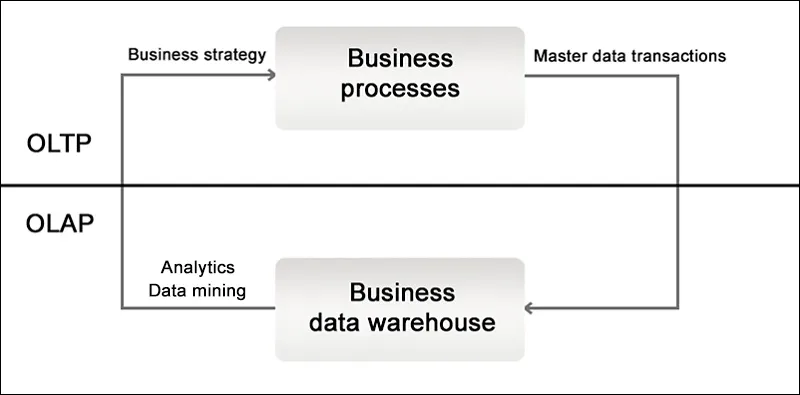
\includegraphics[scale = 0.40]{images/OLAP_OLTP.png}
        \caption{Relation between OLAP and OLTP}
    \end{figure}
    \item {\bfseries What do you mean by cold start problem in collaborative filtering? Explain with example.\\}
    Collaborative filtering is a technique used in recommender systems to provide personalized recommendations to users. In collaborative filtering, the cold start problem refers to the challenge of making accurate recommendations for new users or items who have little to no historical data available in the system. This problem arises because collaborative filtering relies on identifying patterns of similarity between users or items based on their history, and these patterns are difficult to establish for new entities with no prior data.

    For example, let's consider a movie recommendation system that uses collaborative filtering. When a new user signs up for the system, the system has no information about the user's movie preferences, and hence it cannot make any meaningful recommendations for the user. Similarly, when a new movie is added to the system, the system has no information about the movie's genre, actors, or plot, and hence it cannot make any relevant recommendations based on these attributes.
    \item {\bfseries Define the cloud computing and how is it important in MIS? Illustrate types of cloud technology.\\}
    Cloud computing is a model that provides on-demand access to shared computing resources, such as servers, storage, and applications. It is important in MIS because it helps in reducing the cost of managing and maintaining the information system. It provides many benefits, including scalability, flexibility, and cost-effectiveness. There are different types of cloud technology. They are:
    \begin{itemize}
        \item Public cloud: This is a cloud service that is accessible to the public over the internet.
        \item Private cloud: This is a cloud service that is dedicated to a single organization.
        \item Hybrid cloud: This is a cloud service that combines the features of public and private clouds.
    \end{itemize}



    \item {\bfseries Write short notes on:}
    \begin{enumerate}
    \item {\bfseries Balanced Scorecard\\}
    The Balanced Scorecard is a strategic management framework that helps organizations to align their business activities with their strategic goals and objectives. It provides a comprehensive view of an organization's performance by focusing on four perspectives: financial, customer, internal business processes, and learning and growth. By measuring and monitoring these perspectives, organizations can track their progress towards their goals and make informed decisions to improve their performance.
    \item {\bfseries Big-Data processing with Map Reduce\\}
    MapReduce is a programming model and software framework used to process large amounts of data in a distributed and parallel manner. It is typically used in conjunction with the Hadoop Distributed File System (HDFS) to process big data. The MapReduce model consists of two phases: the map phase and the reduce phase. In the map phase, data is divided into smaller chunks and processed in parallel across multiple nodes in a cluster. In the reduce phase, the results from the map phase are combined and processed to produce the final output.
    \item {\bfseries Security Triad\\}
    The Security Triad, also known as the CIA triad, is a framework that helps organizations to ensure the confidentiality, integrity, and availability of their data and information systems. Confidentiality refers to the protection of data from unauthorized access, while integrity refers to the protection of data from unauthorized modification. Availability refers to the ability of authorized users to access data and systems when needed.
    \begin{figure}[h!]
        \centering
        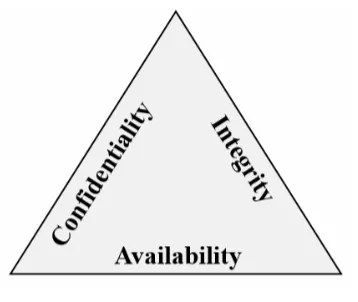
\includegraphics[scale = 0.5]{images/CIA.png}
        \caption{CIA Triad}
    \end{figure}
    \item {\bfseries Collective intelligence through social-network\\}
    Collective intelligence is a concept that describes how groups of individuals can work together to achieve better results than any individual could achieve alone. Social networks are a platform for collective intelligence because they enable individuals to connect and collaborate with others who have similar interests or goals. By sharing information, ideas, and knowledge, social networks can create a collective intelligence that can lead to better decision-making, problem-solving, and innovation.
    \item {\bfseries Knowledge Management System\\}
    Knowledge Management Systems (KMS) are software platforms designed to help organizations manage and share their knowledge and information. KMS typically include features such as document management, search functionality, and collaboration tools to facilitate the creation, storage, and sharing of knowledge within an organization. By capturing and sharing knowledge, organizations can improve their productivity, efficiency, and innovation.
    \item {\bfseries Hadoop System \\}
    Hadoop is an open-source software framework used for distributed storage and processing of big data. It consists of two main components: the Hadoop Distributed File System (HDFS) and the MapReduce programming model. Hadoop allows organizations to store and process large amounts of data across multiple nodes in a cluster, making it an ideal solution for big data processing. Hadoop also provides a number of other tools and frameworks for data processing, such as Pig, Hive, and Spark.
    \end{enumerate}
    \end{enumerate}
    
{\Large 2077 Chaitra}
\begin{enumerate}
    \item {\bfseries What is Information System? What are the differences between IT and IS? Write at least any four types of IS, with brief explanation of each type.\\}
    An information system (IS) is a collection of hardware, software, data, and people that work together to provide important information to an organization. 
    It enables organizations to collect, store, process, and distribute information to support business operations and managerial decision making. 
   
    The differences between IT and IS are: 
    \begin{table}[h!]
        \centering
        \begin{tabular}{|L{6cm}|L{6cm}|}
            \hline
            \textbf{Information Technology (IT)} & \textbf{Information Systems (IS)} \\
            \hline
            Refers to the use of computers, software, and other technologies to manage and process information. & Refers to the broader context in which IT is used to support business processes, decision-making, and strategic planning. \\
            \hline
            Focuses on the technology itself. & Focuses on the use of technology to solve business problems and achieve business goals. \\
            \hline
            Includes hardware, software, and networking technologies that enable the creation, storage, retrieval, and dissemination of information. & Includes people, processes, and technologies that work together to support an organization's information needs. \\
            \hline
            Primarily concerned with the technical aspects of managing and processing information. & Concerned with the broader organizational context in which IT is used. \\
            \hline
            Examples of IT include computer hardware, software applications, networking technologies, and data storage solutions. & Examples of IS include enterprise resource planning (ERP) systems, customer relationship management (CRM) systems, and business intelligence (BI) tools. \\
            \hline
            \end{tabular}
    \end{table}
   
    The different types of information systems are:
    \begin{enumerate}
        \item Transaction Processing System(TPS) : \\
        TPS is a basic information system used to record and process the daily transactions of an organization. It is designed to support middle operational decision making.
        \item Management Information System(MIS) :\\
        MIS is used to provide managers with information that helps them in decision making. It provides reports and summaries of the organization's performance, such as sales reports, inventory reports, and financial reports. It is designed to support middle management decision making.
        \item Decision Support System(DSS) :\\
        DSS is used to support decision making for non-routine and complex problems. It provides tools for analyzing data and making decisions. It is designed to support top management decision making.
        \item Executive Support System(ESS) :\\
        ESS is used to provide executives with information that helps them in decision making. It provides information that is relevant to the organization's strategic objectives. It is designed to support top management decision making.
        \item Office Information System(OIS) :\\
        OIS is used  to help manage documents represented in an electronic format,handle messages, such as e-mail, facsimile and voice mail, handle teleconferencing and electronic meetings and so on. It is designed to facilitate communication between the members of an organization and between the organization and its environment.
    \end{enumerate}
    \item {\bfseries Mention any three levels of securities that could be implemented while building any IS with brief explanation. Is 'Security Policy' same as 'Security Method'? Justify your argument with appropriate example of IS implementation scenario.\\}
   Information security is an essential aspect of any organization's operations. An organization must ensure that its information systems are secure to maintain the confidentiality, integrity, and availability of its data. The three levels of security that could be implemented while building any IS are:
   \begin{itemize}
    \item Physical security: \\This includes measures such as access controls, surveillance systems, and alarm systems to protect the physical assets of the organization.
    \item Network security:\\ This includes measures such as firewalls, intrusion detection systems, and virtual private networks (VPNs) to protect the organization's network from external threats.
    \item  Operating system security:\\ This includes measures such as user authentication, access controls, and antivirus software to protect the operating system from internal and external threats.
    \item Application security: This includes measures such as secure coding practices, input validation, and encryption to protect the organization's applications from external threats.
\end{itemize}

A security policy is a set of guidelines and procedures that are designed to protect an organization's information systems and data. A security method, on the other hand, is a specific technique or tool that is used to implement the security policy. The security policy provides the framework for implementing security measures, while the security method provides the specific tools and techniques that are used to implement the policy.

For example, an IS implementation scenario could involve the development of a security policy to protect customer data. The security policy could include guidelines for access controls, data encryption, and backup procedures. The security method could involve the use of a firewall, antivirus software, and intrusion detection systems to implement the security policy.
    \item {\bfseries What is the hierarchical relationship among data, information and knowledge (DIK)?Establish DIK linkages associating with domain and system knowledges. Illustrate all in single diagram.\\}
    Data, information, and knowledge (DIK) are related concepts that form a hierarchy. Data is the raw facts and figures that are collected and stored. Information is the processed data that is organized and presented in a meaningful way. Knowledge is the understanding and insights that are gained from the information.

The relationship between data, information, and knowledge can be illustrated in following single diagram:
\begin{figure}[h!]
    \centering
    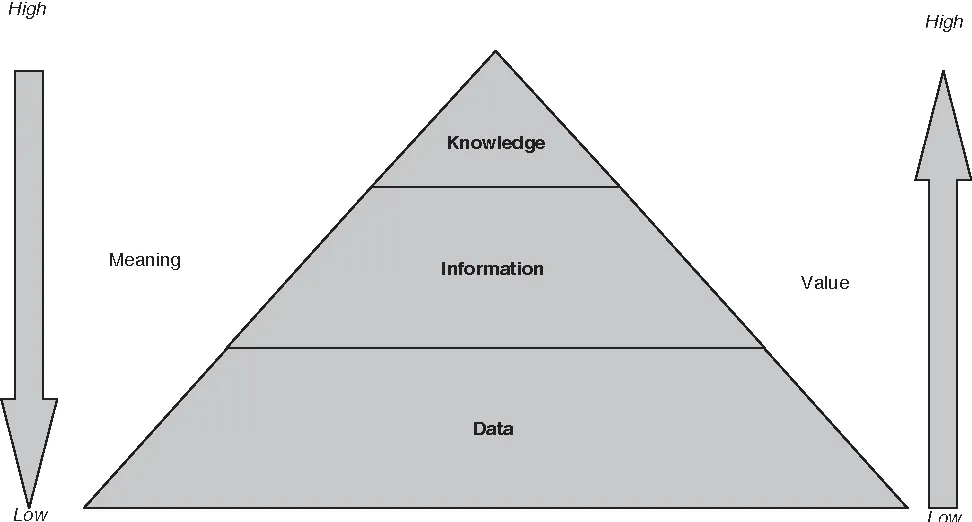
\includegraphics[scale=0.3]{images/DIK.png}
    \caption{DIK hierarchy}
\end{figure}

In this hierarchy, data is the lowest level, followed by information, and then knowledge. Data is processed to create information, and information is used to create knowledge. 
    \item {\bfseries Why change management is required? What are the key principles of change management? Write briefly within IS context.\\}
    Change management is crucial for any modern organization because it helps in managing the transition from the current state to the desired state. Change management involves the process of preparing, equipping, and supporting individuals to adopt a new system or process. Effective change management can help to minimize resistance to change, reduce the time required for adoption, and increase the chances of success.

The key principles of change management are:

\begin{itemize}
\item Clear communication: Effective communication is essential for ensuring that everyone understands why the change is necessary, what the change involves, and how it will affect them.
\item Employee involvement: Employees should be involved in the change process to ensure that their concerns are addressed and that they have a sense of ownership in the process.
\item Leadership support: Change management requires the support of top management to ensure that the necessary resources are available and that everyone is committed to the change.
\item Training and education: Users need to be trained on how to use the new system effectively. Without proper training, the system may not be used to its full potential, and the benefits may not be realized.
\item Continuous improvement: Change management is an ongoing process that requires continuous improvement. Feedback should be solicited and analyzed to identify areas for improvement.
\end{itemize}
    \item {\bfseries What is a recommender system? How does a collaborative filtering method generate potential recommendations? Explain in brief with sample example.\\}
    A recommender system is a software tool that provides personalized recommendations to users based on user's past interaction with the software. 
    
    Collaborative filtering is a technique used in recommender systems to generate potential recommendations. Collaborative filtering works by identifying users with similar preferences and making recommendations based on the items that they have rated or purchased.
    
    For example, suppose that a user has rated several movies on a movie streaming service. Collaborative filtering would identify other users who have rated the same movies and compare their ratings with the user's ratings. Based on this comparison, collaborative filtering would generate potential movie recommendations for the user.
    \item {\bfseries Define cloud computing. Why cloud computing knowledge is becoming as an essential for any seasoned IS designing professional? Justify.\\}
    Cloud computing is a model that provides on-demand access to shared computing resources, such as servers, storage, and applications. Cloud computing is important in MIS because it helps in reducing the cost of managing and maintaining the information system.
    
    Cloud computing provides many benefits, including scalability, flexibility, and cost-effectiveness. Thus, cloud computing knowledge is becoming essential for any seasoned IS designing professional because of the increasing use of cloud technology in modern organizations. IS designing professionals need to have a good understanding of cloud computing to design and implement cloud-based solutions that meet the organization's needs. They need to be able to evaluate the different types of cloud technology and determine which one is the best fit for the organization. They also need to be able to design cloud-based solutions that are secure, scalable, and cost-effective.
    \item {\bfseries What is CRM? How closely CRM is associated with SCM? Why SCM and CRM are becoming important in e-commerce in comparison to regular brick-and-mortar commerce?\\}
    CRM stands for Customer Relationship Management. CRM is a strategy that is used to manage interactions with customers and improve customer satisfaction. It involves using technology to organize, automate, and synchronize sales, marketing, customer service, and technical support processes.
    
    SCM stands for Supply Chain Management. It involves the management of the flow of goods, services, and information from the suppliers to the customers. It helps organizations to improve the efficiency of the supply chain, reduce costs, and improve customer satisfaction.
    
    CRM and SCM are closely associated because they both focus on improving customer satisfaction. CRM helps organizations to manage interactions with customers, while SCM helps organizations to manage interactions with suppliers. Together, CRM and SCM help organizations to create a seamless customer experience that meets the needs of both the customer and the organization.
    
    SCM and CRM are becoming important in e-commerce in comparison to regular brick-and-mortar commerce because of the unique challenges presented by e-commerce. In e-commerce, customers are often located in different parts of the world, and suppliers may be located in different countries. This makes it difficult to manage the supply chain and to provide effective customer service. SCM and CRM provide the tools and processes that are necessary to manage these challenges and to provide a seamless customer experience.
    \item {\bfseries Compare and contrast the followings:}
    \begin{enumerate}
        \item {\bfseries Fully integrated vs Loosely integrated enterprises}
        \begin{longtable}{|p{6cm}|p{6cm}|}
                \hline
                \textbf{Fully Integrated Enterprises} & \textbf{Loosely Integrated Enterprises} \\
                \hline
                They are organizations that have tightly controlled and coordinated business processes that are integrated across all departments and functions. & They are organizations that have more flexible and decentralized business processes that may not be fully integrated across all departments and functions. \\
                \hline
                They typically have a single centralized database or information system that supports all business processes and functions. & They may have multiple databases or information systems that support different business processes and functions. \\
                \hline
                They are highly standardized and have consistent processes and procedures across all departments and functions. & They are less standardized and may have different processes and procedures across different departments and functions. \\
                \hline
                They have a high degree of control over their operations and are less reliant on external partners or suppliers. & They rely more on external partners or suppliers to provide goods and services that they may not have in-house. \\
                \hline
                They are more suited for organizations with highly predictable and stable environments where standardization and control are important. & They are more suited for organizations with dynamic and changing environments where flexibility and adaptation are important. \\
                \hline
                Examples of fully integrated enterprises include manufacturing and production companies that use just-in-time inventory management systems, where all processes are tightly integrated and controlled. & Examples of loosely integrated enterprises include technology companies that use agile development methodologies, where different teams work on different aspects of a project and may have different processes and procedures. \\
                \hline
        \end{longtable}
        \item {\bfseries CSF vs KPI}
        \begin{longtable}{|p{6cm}|p{6cm}|}
            \hline
            \textbf{Critical Success Factors (CSF)} & \textbf{Key Performance Indicators (KPI)} \\
            \hline
            Critical Success Factors are the essential areas that must be focused on for an organization to achieve its goals and objectives. & Key Performance Indicators are the measurable values that indicate how well an organization is achieving its goals and objectives. \\
            \hline
            CSFs are qualitative in nature and are used to identify the key drivers of success for an organization. & KPIs are quantitative in nature and are used to measure the progress of an organization towards its goals and objectives. \\
            \hline
            They are strategic in nature and are used to guide decision-making and resource allocation. & They are tactical in nature and are used to monitor performance and make adjustments as needed. \\
            \hline
            They are often unique to each organization and reflect its specific industry, market, and competitive environment. & They are often more standardized and can be used across different organizations and industries. \\
            \hline
            They are typically focused on long-term outcomes and are used to evaluate the overall health and success of an organization. & They are typically focused on short-term outcomes and are used to evaluate the performance of specific processes or functions. \\
            \hline
            Examples of CSFs may include customer satisfaction, employee engagement, or innovation. & Examples of KPIs may include sales revenue, customer retention rate, or on-time delivery rate. \\
            \hline
            \label{tab:csf-kpi}
            \end{longtable}
        \item {\bfseries Web content mining vs Web uses mining}
        \begin{longtable}{|p{6cm}|p{6cm}|}
            \hline
            \textbf{Web Content Mining} & \textbf{Web Usage Mining} \\
            \hline
            Web Content Mining is the process of extracting useful information and knowledge from web content, including text, images, videos, and audio. & Web Usage Mining is the process of analyzing user behavior and interactions with web-based systems, such as websites, online applications, and social media platforms. \\
            \hline
            It involves techniques such as text mining, image mining, and multimedia mining to identify patterns and insights in web content. & It involves techniques such as clickstream analysis, path analysis, and session clustering to understand how users navigate and use web-based systems. \\
            \hline
            Web Content Mining is useful for tasks such as content categorization, sentiment analysis, and search engine optimization. & Web Usage Mining is useful for tasks such as website optimization, personalization, and marketing campaign optimization. \\
            \hline
            It focuses on the static aspects of web content, such as the information that is presented on a website or web page. & It focuses on the dynamic aspects of user behavior, such as how users interact with web-based systems over time. \\
            \hline
            Web Content Mining is more suited for tasks that require a deep understanding of the content itself, such as natural language processing or image recognition. & Web Usage Mining is more suited for tasks that require an understanding of how users interact with web-based systems, such as user experience design or customer journey mapping. \\
            \hline
            Examples of Web Content Mining applications include news aggregation, e-commerce product recommendations, and social media analysis. & Examples of Web Usage Mining applications include website analytics, user profiling, and clickstream analysis. \\
            \hline
            \end{longtable}
        \item {\bfseries MapReduce vs Hadoop system}
        \begin{longtable}{|p{6cm}|p{6cm}|}
            \hline
            \textbf{MapReduce} & \textbf{Hadoop} \\
            \hline
            MapReduce is a programming model for processing large data sets across a cluster of computers. & Hadoop is an open-source software framework that provides a distributed storage and processing system for big data applications. \\
            \hline
            It is designed to work with a wide variety of data processing tasks, including batch processing, data mining, and machine learning. & It is designed to handle massive amounts of data, both structured and unstructured, and to provide reliable and scalable distributed computing. \\
            \hline
            MapReduce breaks down large data sets into smaller chunks, and processes them in parallel across a cluster of computers. & Hadoop uses the Hadoop Distributed File System (HDFS) to store data across multiple nodes in a cluster, and the MapReduce programming model to process that data in parallel. \\
            \hline
            MapReduce consists of two phases: the map phase, which processes input data and produces a set of intermediate key-value pairs, and the reduce phase, which aggregates the intermediate data to produce the final output. & Hadoop includes several components, such as HDFS, YARN, and MapReduce, that work together to provide a complete distributed processing system. \\
            \hline
            MapReduce is typically used in conjunction with other technologies, such as Hadoop, to process large data sets efficiently. & Hadoop is widely used in big data applications, such as log processing, social media analysis, and financial analysis. \\
            \hline
            Examples of MapReduce applications include word count, data cleansing, and sentiment analysis. & Examples of Hadoop applications include Hadoop MapReduce, Hadoop Streaming, and Hadoop Pig. \\
            \hline
            \end{longtable}
    \end{enumerate}
    \item {\bfseries Write short notes on the followings:}
    \begin{enumerate}
        \item {\bfseries ERP System in large organization\\}
        ERP stands for Enterprise Resource Planning. Itis a type of software system used by large organizations to manage and integrate their core business processes. ERP systems typically include modules for managing areas such as finance, accounting, human resources, supply chain management, and customer relationship management. In a large organization, an ERP system can help to standardize and streamline business processes across multiple departments and locations. This can lead to improved efficiency, better visibility into business operations, and more accurate reporting and analysis. However, implementing an ERP system can be a complex and expensive undertaking, requiring significant changes to existing business processes and IT infrastructure. Successful implementation typically requires strong project management, extensive planning and testing, and close collaboration between IT and business stakeholders.
        \item {\bfseries CIA Triangle\\}
        The Security Triad, also known as the CIA triad, is a framework that helps organizations to ensure the confidentiality, integrity, and availability of their data and information systems. Confidentiality refers to the protection of data from unauthorized access, while integrity refers to the protection of data from unauthorized modification. Availability refers to the ability of authorized users to access data and systems when needed.
    \begin{figure}[h!]
        \centering
        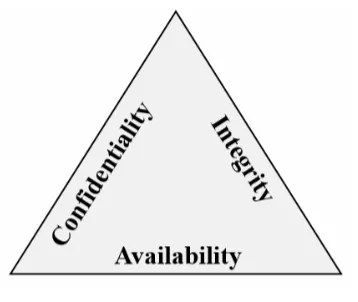
\includegraphics[scale = 0.5]{images/CIA.png}
        \caption{CIA Triad}
    \end{figure}
        \item {\bfseries Collective intelligence through social network\\}
        Collective intelligence is a concept that describes how groups of individuals can work together to achieve better results than any individual could achieve alone. Social networks are a platform for collective intelligence because they enable individuals to connect and collaborate with others who have similar interests or goals. By sharing information, ideas, and knowledge, social networks can create a collective intelligence that can lead to better decision-making, problem-solving, and innovation.
        \item {\bfseries Big- Data processing with MapReduce\\}
        Big Data processing with MapReduce is a popular technique used to process and analyze large amounts of data in a distributed computing environment. MapReduce is a programming model and framework originally developed by Google that allows for parallel processing of large datasets across a cluster of computers. In MapReduce, data is split into small chunks and distributed across multiple computers in the cluster. Each computer independently processes the data and produces intermediate results, which are then combined to produce the final output. The framework consists of two main phases: Map and Reduce. The Map phase involves processing each data item in parallel across multiple computers, transforming the input data into a set of key-value pairs. The key-value pairs are then shuffled and sorted to group together similar items. In the Reduce phase, the grouped key-value pairs are processed in parallel across multiple computers, performing a set of operations such as aggregation, filtering, or sorting. The final output is then written to a storage system, such as a database or a file system.MapReduce is commonly used in Big Data applications, such as processing large datasets from social media, web logs, or sensor networks. It is also used in applications that require real-time processing, such as fraud detection or recommendation systems.
    \end{enumerate}
\end{enumerate}
\pagebreak
{\Large 2075 Bhadra}
\begin{enumerate}
    \item {\bfseries Some people say, 'Information is always costlier than hardware'. Do you agree or disagree? In any case, justify your argument, providing some relevant examples too.\\}
    In the modern era, we live in a world where data is constantly generated, and organizations across industries are constantly collecting, storing, and analyzing large amounts of data to derive insights and make informed decisions. As such, information has become a valuable asset for organizations, often more so than hardware.

While hardware is necessary for processing and storing data, it is only as valuable as the information it can process. Without valuable data, hardware would have little use. On the other hand, the right information can help organizations make more informed decisions, optimize processes, and gain a competitive advantage.

For example, consider a healthcare organization that has invested in state-of-the-art medical equipment but lacks a centralized database to store and analyze patient data. The equipment alone would be of little use if the organization cannot utilize the data it generates. In contrast, if the organization had a centralized database that could analyze patient data, it could derive insights to improve patient outcomes and optimize resource utilization.
    \item {\bfseries What do you mean by extended validation? How can you recognize websites using EV and SSL certificates?\\}
    Extended Validation (EV) is a type of SSL/TLS certificate that provides an additional level of validation and authentication for websites. It involves a rigorous verification process to confirm the identity of the website owner, and as a result, it is considered more secure than regular SSL/TLS certificates.

To recognize websites using EV and SSL certificates, users can look for visual cues in their web browser's address bar. When a website uses an EV certificate, the browser will display a green padlock icon and the company name in the address bar. This indicates that the website has undergone a thorough validation process and that the connection is encrypted and secure.

Additionally, users can check the certificate details by clicking on the padlock icon in the address bar and selecting "Certificate". This will display information about the certificate issuer, expiration date, and other details. For EV certificates, the certificate details will also include the company name and location, providing further assurance of the website's authenticity.
    
\item {\bfseries What are typical characteristics that a systems designer has to look for in any Enterprise Management System? Write in detail with the three different system references of ERP, SCM, and CRM.\\}
An Enterprise Management System (EMS) is a comprehensive software solution that assists in automating and integrating a variety of business processes across different functional areas of an organization. A systems designer needs to consider several characteristics while designing an EMS to ensure its effective implementation and utilization. Some typical characteristics of an EMS are:
\begin{enumerate}
    \item \textbf{Flexibility:} The EMS should be flexible enough to adapt to changing business needs and processes. It should support customization and configuration options to meet the specific requirements of an organization.
    

    \item \textbf{Scalability:} The EMS should be scalable enough to handle the increasing volumes of data and transactions as the organization grows. It should support the addition of new modules and functionalities without disrupting the existing system.
    
    \item \textbf{Reliability:} The EMS should be highly reliable and available at all times, as any downtime can result in significant business losses. It should have a robust backup and recovery mechanism to ensure the safety and integrity of data.
    
    \item \textbf{Integration:} The EMS should be capable of integrating with other systems and applications within the organization. It should allow for seamless exchange of data and information across different functional areas.
    
    \item \textbf{Security:} The EMS should have robust security features to ensure the confidentiality, integrity, and availability of data. It should support access control mechanisms to restrict unauthorized access to sensitive data.
    
    \item \textbf{Usability:} The EMS should be easy to use and intuitive, with a user-friendly interface that requires minimal training. It should provide relevant information in a timely and actionable manner to support decision-making.
    \end{enumerate}
    
    There are three different types of Enterprise Management Systems, namely ERP, SCM, and CRM. Each of these systems has its own set of functionalities and characteristics.
    
    \begin{enumerate}
    \item \textbf{Enterprise Resource Planning (ERP):} ERP is a system that integrates and automates all business processes, including finance, accounting, human resources, procurement, inventory, and customer relationship management, into a single system. An ERP system provides a comprehensive view of the entire organization, allowing for better decision-making, improved operational efficiency, and reduced costs. Some key characteristics of an ERP system are centralization of data, process standardization, and real-time information.
    
    \item \textbf{Supply Chain Management (SCM):} SCM is a system that manages the entire process of the supply chain, from the procurement of raw materials to the delivery of finished products to customers. SCM aims to optimize the supply chain by minimizing costs, improving quality, and reducing lead times. Some key characteristics of an SCM system are supply chain visibility, demand forecasting, and inventory management.
    
    \item \textbf{Customer Relationship Management (CRM):} CRM is a system that manages the entire customer life cycle, from lead generation to customer retention. CRM aims to improve customer satisfaction and loyalty by providing personalized and efficient customer service. Some key characteristics of a CRM system are customer data management, sales automation, and marketing automation.
    \end{enumerate}
    \item {\bfseries What do you mean by data mining? How is it related to data warehouse? Differentiate OLAP and OLTP.\\}
    Data mining refers to the process of discovering patterns, trends, and relationships within large datasets using various statistical and machine learning techniques. It involves extracting valuable insights and knowledge from data that may not be immediately apparent.

Data mining is related to data warehouse in the sense that data warehouses are typically used as the primary source of data for data mining. A data warehouse is a large, centralized repository of integrated data from various sources within an organization. The data within a data warehouse is typically structured and organized in a way that allows for efficient querying and analysis.

OLAP (Online Analytical Processing) and OLTP (Online Transaction Processing) are two types of systems that are commonly used in conjunction with data mining and data warehousing.
    {\centering \begin{longtable}{ |L{3cm}|L{4.5cm}|L{4.5cm}| }
        \hline
        Basis& OLAP & OLTP \\
        \hline
        Stands for & Online Analytical Processing & Online Transaction Processing \\
        \hline
        Purpose & Provides business intelligence & Supports transaction processing \\
        \hline
        Data type & Historical data & Current, real-time data \\
        \hline
        Database structure & Multidimensional & Relational \\
        \hline
        Data query & Complex & Simple \\
        \hline
        Query response time & Slow & Fast \\
        \hline
        Usage & Decision making & Daily operations \\
        \hline
        Examples & Data warehousing, business intelligence & Retail sales, banking transactions \\
        \hline
        \end{longtable}}
\item {\bfseries The famous bank in town, Chuchche Bank, has DSS built onto the FMS, which automatically estimates the cash amount required for the next day to get from the central treasury for every branch of the bank, during the end-of-day processing. Present the design and DFDs of such DDS in detail. Clearly state the assumptions that you are going to make on the availability of data and other constraints, first.}
    
\item {\bfseries Explain Change Management. What are different change management tactics that are to be applied during the execution of change management?\\}
Change management is a structured approach to transition individuals, teams, and organizations from their current state to a desired future state. It involves the processes, tools, and techniques used to manage the people side of change and ensure successful adoption of new processes, technologies, or strategies. Change management helps to minimize the negative impacts of change on individuals and teams, and maximize the benefits of the change initiative for the organization as a whole.
\begin{itemize}

There are several change management tactics that can be applied during the execution of change management. Some of these include:
    \item \textbf{Communication}: Effective communication is critical during change management. It is important to clearly communicate the reasons for the change, the expected outcomes, and the impact on individuals and teams.
    
    \item \textbf{Training and education}: Providing training and education to employees can help them understand the new processes and technologies, and prepare them for their new roles and responsibilities.
    
    \item \textbf{Change champions}: Identifying change champions within the organization can help to promote the change initiative and encourage others to adopt the new processes or technologies.
    
    \item \textbf{Piloting}: Piloting the change initiative in a small-scale environment before rolling it out across the entire organization can help to identify any issues or challenges and allow for adjustments to be made before the full implementation.
    
    \item \textbf{Rewards and recognition}: Providing rewards and recognition for employees who successfully adopt the new processes or technologies can help to reinforce positive behavior and encourage others to follow suit.
    
    \item \textbf{Resistance management}: Addressing resistance to change is a critical aspect of change management. Understanding the reasons for resistance and providing support and resources to overcome it can help to ensure the success of the change initiative.
    \end{itemize}
    \item {\bfseries Prepare a brief note on 'cloud computing' with clear statements on associated technologies, their types, and various issues.\\}
    Cloud computing is a technology that allows users to access computing resources, such as servers, storage, and applications, over the internet. 
    
    There are several technologies associated with Cloud computing. They are:
    \begin{itemize}
        \item Virtualization: enables multiple operating systems to run on a single physical machine, allowing for more efficient use of resources.
        \item Containerization: a lightweight alternative to virtualization that allows for the creation of portable and scalable software packages.
        \item Distributed computing: the use of multiple computers to perform a single task or set of tasks, resulting in faster processing times.
        \item Automation: the use of software tools to automate tasks such as deployment, scaling, and maintenance, reducing the need for manual intervention.
    \end{itemize}
    
    There are several types of cloud computing, including:
    \begin{itemize}
        \item Infrastructure as a Service (IaaS):\\ This type of cloud computing provides users with access to computing resources like virtual machines, storage, and networks. Users are responsible for managing the operating systems, applications, and data that run on these resources.
        \item Platform as a Service (PaaS):\\ This type of cloud computing provides users with a platform to develop, run, and manage applications without having to worry about the underlying infrastructure. The provider manages the infrastructure, and users only need to focus on their applications.
        \item Software as a Service (SaaS):\\ This type of cloud computing provides access to software applications over the internet.
    \end{itemize}

Issues related to cloud computing include concerns about data security and privacy, the reliability of cloud services, and the potential for vendor lock-in.
\begin{itemize}
    \item Security and Privacy: as data is stored offsite and accessed over the internet, there is a risk of data breaches, hacking, and other security issues.
    \item Vendor Lock-In: users may become dependent on a single cloud provider and find it difficult to switch to another provider due to differences in technology and data formats.
    \item Reliability: cloud computing relies on the availability of internet connections and the performance of cloud providers' infrastructure, which can affect the reliability of the service.
    \item Cost: while cloud computing can save costs by reducing the need for hardware and software infrastructure, it can also result in unexpected expenses due to factors such as data transfer fees and usage limits.
\end{itemize}
    \item {\bfseries Discuss Tactical Operational Information Systems and Strategic.\\}
    Tactical Operational Information Systems (TOIS) are information systems that support the day-to-day operations of an organization. They are designed to support the operational decision-making needs of managers and staff who are responsible for the daily operations of the organization. Examples of TOIS include transaction processing systems, office automation systems, and decision support systems.
    
    Strategic Information Systems (SIS) are information systems that are designed to support the strategic goals and objectives of an organization. They are used to gain a competitive advantage, support decision-making at the executive level, and create new products and services. Examples of SIS include executive support systems, enterprise resource planning systems, and knowledge management systems.
    
    The differences between TOIS and SIS are summarized in the following table:

\begin{longtable}{|p{6cm}|p{6cm}|}
\hline
\textbf{Tactical Operational Information Systems (TOIS)} & \textbf{Strategic Information Systems (SIS)} \\
\hline
Designed to support the day-to-day operations of an organization. & Designed to support the strategic goals and objectives of an organization. \\
\hline
Used to support the operational decision-making needs of managers and staff who are responsible for the daily operations of the organization. & Used to support decision-making at the executive level. \\
\hline
Examples include transaction processing systems, office automation systems, and decision support systems. & Examples include executive support systems, enterprise resource planning systems, and knowledge management systems. \\
\hline
Focused on improving operational efficiency and effectiveness. & Focused on gaining a competitive advantage and creating new products and services. \\
\hline
Data used by TOIS is typically operational or transactional data. & Data used by SIS is typically strategic or external data. \\
\hline
\end{longtable}
    \item {\bfseries Write short notes on the following:}
    \begin{enumerate}
    \item {\bfseries Big-data processing using Hadoop system\\}
    Big data processing refers to the handling of massive amounts of data that cannot be processed using traditional data processing techniques. Hadoop is an open-source software framework that is designed to handle big data processing. It is widely used for storing and processing large volumes of data across a distributed computing infrastructure.

    The Hadoop system is comprised of two main components: the Hadoop Distributed File System (HDFS) and MapReduce. HDFS is a distributed file system that provides high-throughput access to data across multiple nodes in a Hadoop cluster. MapReduce is a programming model that enables the processing of large datasets across a distributed computing infrastructure.
    
    The Hadoop system is designed to be highly scalable and fault-tolerant. It can handle petabytes of data and can run on commodity hardware. The Hadoop system is also designed to be cost-effective, as it allows organizations to store and process large volumes of data without the need for expensive hardware and software infrastructure.
    
    To process data using the Hadoop system, data is first stored in the HDFS. The data is then processed using MapReduce, which divides the data into smaller chunks and distributes them across the nodes in the Hadoop cluster. Each node processes its assigned chunk of data and produces intermediate results, which are then combined to produce the final output.
    
    Hadoop also provides a number of tools and libraries for data processing, such as Pig, Hive, and Spark. These tools provide higher-level abstractions for data processing, making it easier for developers to write and execute data processing tasks.
    
    One of the key benefits of using Hadoop for big data processing is its ability to handle unstructured and semi-structured data, such as text, images, and video. This makes it an ideal platform for processing data from social media, web logs, and other sources of unstructured data.
    
    In summary, the Hadoop system is a powerful and scalable platform for big data processing. It provides a distributed file system and a programming model for processing large volumes of data across a distributed computing infrastructure. The Hadoop system is widely used in industry for a variety of big data processing applications.
    \item {\bfseries Collective intelligence through social-network\\}
    Collective intelligence is a concept that describes how groups of individuals can work together to achieve better results than any individual could achieve alone. Social networks are a platform for collective intelligence because they enable individuals to connect and collaborate with others who have similar interests or goals. By sharing information, ideas, and knowledge, social networks can create a collective intelligence that can lead to better decision-making, problem-solving, and innovation.
    \item {\bfseries Link analysis as web structure mining\\}
    Link analysis is a technique used in web structure mining to analyze the relationships between pages on the web. It involves examining the links between web pages to identify patterns, trends, and relationships that can be used to understand the structure of the web.

Link analysis is used in a number of different applications, including search engine optimization, fraud detection, and social network analysis. In search engine optimization, link analysis is used to understand the importance of a web page by analyzing the links that point to it. In fraud detection, link analysis is used to identify patterns of fraudulent behavior by analyzing the links between individuals or organizations. In social network analysis, link analysis is used to understand the structure of social networks by analyzing the links between individuals.

Link analysis is typically performed using graph theory, which is a mathematical framework for analyzing relationships between objects. In web structure mining, the web is represented as a graph, with web pages as nodes and links between them as edges. By analyzing the structure of this graph, link analysis can reveal important information about the web, such as which pages are the most important or which pages are the most connected.
    \item {\bfseries Critical success factors of IS\\}
    Critical Success Factors(CSF) are the key areas that an organization must focus on to achieve its objectives. CSF can vary depending on the organization's field, size, and objectives. Some of the common CSF include:
        \begin{itemize}
            \item Customer satisfaction
            \item Quality of products and services
            \item Employee satisfaction and engagement
            \item Financial performance
        \end{itemize}
    \end{enumerate}
    \end{enumerate}
    \pagebreak
{\Large 2075 Magh}
\begin{enumerate}
    \item {\bfseries What is an Information system? How it is different from Information Technology?
    Explain the types of IS used in an organization.\\}
    An information system (IS) is a collection of hardware, software, data, and people that work together to provide important information to an organization. 
    It enables organizations to collect, store, process, and distribute information to support business operations and managerial decision making. 
   
    The differences between IT and IS are: 
    \begin{table}[h!]
        \centering
        \begin{tabular}{|L{6cm}|L{6cm}|}
            \hline
            \textbf{Information Technology (IT)} & \textbf{Information Systems (IS)} \\
            \hline
            Refers to the use of computers, software, and other technologies to manage and process information. & Refers to the broader context in which IT is used to support business processes, decision-making, and strategic planning. \\
            \hline
            Focuses on the technology itself. & Focuses on the use of technology to solve business problems and achieve business goals. \\
            \hline
            Includes hardware, software, and networking technologies that enable the creation, storage, retrieval, and dissemination of information. & Includes people, processes, and technologies that work together to support an organization's information needs. \\
            \hline
            Primarily concerned with the technical aspects of managing and processing information. & Concerned with the broader organizational context in which IT is used. \\
            \hline
            Examples of IT include computer hardware, software applications, networking technologies, and data storage solutions. & Examples of IS include enterprise resource planning (ERP) systems, customer relationship management (CRM) systems, and business intelligence (BI) tools. \\
            \hline
            \end{tabular}
    \end{table}
   
    The different types of information systems are:
    \begin{enumerate}
        \item Transaction Processing System(TPS) : \\
        TPS is a basic information system used to record and process the daily transactions of an organization. It is designed to support middle operational decision making.
        \item Management Information System(MIS) :\\
        MIS is used to provide managers with information that helps them in decision making. It provides reports and summaries of the organization's performance, such as sales reports, inventory reports, and financial reports. It is designed to support middle management decision making.
        \item Decision Support System(DSS) :\\
        DSS is used to support decision making for non-routine and complex problems. It provides tools for analyzing data and making decisions. It is designed to support top management decision making.
        \item Executive Support System(ESS) :\\
        ESS is used to provide executives with information that helps them in decision making. It provides information that is relevant to the organization's strategic objectives. It is designed to support top management decision making.
        \item Office Information System(OIS) :\\
        OIS is used  to help manage documents represented in an electronic format,handle messages, such as e-mail, facsimile and voice mail, handle teleconferencing and electronic meetings and so on. It is designed to facilitate communication between the members of an organization and between the organization and its environment.
    \end{enumerate}
    \item {\bfseries What is authentication? Does SSL based implementation augment the security of any IS? Why SSL is also paired with TLS in most of the documentation? Prepare a detail on SSL.\\}
    Authentication is the process of verifying the identity of a user, device, or system. In the context of information security, authentication is a critical component of access control, which ensures that only authorized users, devices, or systems are granted access to sensitive information or resources. Authentication can be performed using various techniques, including passwords, biometric authentication, smart cards, and digital certificates. These techniques are designed to ensure that the user or device attempting to access the system is who they claim to be.

    SSL (Secure Sockets Layer) is a cryptographic protocol that is used to secure communications over the internet. It provides authentication, encryption, and integrity protection for data transmitted between web servers and clients, such as web browsers. SSL is based on a public-key infrastructure, which means that it uses digital certificates to authenticate the identity of web servers and clients. These digital certificates are issued by trusted third-party organizations called Certificate Authorities (CAs). When a user connects to a web server using SSL, the server presents its digital certificate to the client, which then verifies the certificate using the CA's public key. This process ensures that the client is communicating with the authentic server and not an imposter. SSL provides several benefits for information security. It encrypts data transmitted between the client and server, which ensures that sensitive information, such as passwords and credit card numbers, cannot be intercepted by attackers. It also provides integrity protection, which ensures that data cannot be tampered with during transmission.
    
    SSL has since been replaced by the newer TLS (Transport Layer Security) protocol, which is an updated version of SSL. However, the term SSL is still commonly used to refer to both SSL and TLS.SSL and TLS are often paired in documentation because they are both used to secure communications over the internet. TLS is considered a more secure protocol than SSL and is used in newer implementations. However, SSL is still widely used, particularly in older systems and applications.
\item {\bfseries Explain Enterprise Management Systems? Discuss its Architecture. Explain the role of IS and IT in enterprise management.\\}
Enterprise Management Systems (EMS) are software applications that help organizations manage their day-to-day operations and facilitate the decision-making process. These systems are designed to integrate various business processes, such as finance, human resources, marketing, and operations, into a single, unified platform.

The architecture of an EMS typically consists of three layers: the presentation layer, the application layer, and the data layer. The presentation layer is the user interface that allows users to interact with the system. The application layer contains the business logic and processes that govern how the system works. The data layer contains the databases that store the organization's data.

The role of Information Systems (IS) and Information Technology (IT) in enterprise management is significant. IS is responsible for designing, implementing, and maintaining the software applications that are used to manage business operations. IT is responsible for providing the necessary hardware, networking, and infrastructure to support the IS applications. IS and IT work together to ensure that the EMS meets the organization's needs and requirements. They collaborate with other departments, such as finance, human resources, and marketing, to understand their business processes and design solutions that streamline their operations and improve their efficiency. IS and IT also play a critical role in maintaining the security and integrity of the EMS. They implement security measures, such as firewalls, access controls, and encryption, to protect the system from unauthorized access and data breaches. They also monitor the system for vulnerabilities and take proactive measures to address any security risks that are identified.

\item {\bfseries What are the benefits of Cloud Computing? Explain different types of Cloud Computing.\\}
Cloud computing is a model that provides on-demand access to shared computing resources, such as servers, storage, and applications. Cloud computing provides many benefits, including scalability, flexibility, and cost-effectiveness. 
\begin{itemize}
    \item Scalability: Cloud computing allows for the easy scaling of resources up or down as needed, without the need for physical infrastructure changes.
    \item Cost-effectiveness: Cloud computing can be more cost-effective for businesses as it reduces the need for investing in and maintaining physical hardware and infrastructure.
    \item Accessibility: Cloud computing allows for easy access to data and applications from anywhere with an internet connection, making it more accessible for remote workers and teams.
    \item Flexibility: Cloud computing offers flexibility in terms of the types of applications and services that can be deployed, as well as the ability to easily switch between different services or providers.
    \item Security: Cloud providers often have more advanced security measures in place to protect data, applications, and infrastructure, than most businesses could implement themselves.
    \item Collaboration: Cloud computing allows for easy collaboration between teams and individuals working on the same project or application, regardless of location.
    \item Disaster recovery: Cloud providers often have robust disaster recovery and backup solutions in place, helping businesses to recover data and applications in the event of a disaster or outage.
    \item Environmentally friendly: Cloud computing can help reduce the carbon footprint of businesses by reducing the need for physical hardware and infrastructure, and enabling more energy-efficient data centers.
    \end{itemize}

There are several types of cloud computing, including:
    \begin{itemize}
        \item Infrastructure as a Service (IaaS):\\ This type of cloud computing provides users with access to computing resources like virtual machines, storage, and networks. Users are responsible for managing the operating systems, applications, and data that run on these resources.
        \item Platform as a Service (PaaS):\\ This type of cloud computing provides users with a platform to develop, run, and manage applications without having to worry about the underlying infrastructure. The provider manages the infrastructure, and users only need to focus on their applications.
        \item Software as a Service (SaaS):\\ This type of cloud computing provides access to software applications over the internet.
    \end{itemize}
    \item{\bfseries Differentiate among the following with multiple aspect/feature distinction}
    \begin{enumerate}
        \item {\bfseries OLTP vs OLAP}
        { \begin{longtable}{ |C{3cm}|L{4.5cm}|L{4.5cm}| }
            \hline
            Basis& OLAP & OLTP \\
            \hline
            Stands for & Online Analytical Processing & Online Transaction Processing \\
            \hline
            Purpose & Provides business intelligence & Supports transaction processing \\
            \hline
            Data type & Historical data & Current, real-time data \\
            \hline
            Database structure & Multidimensional & Relational \\
            \hline
            Data query & Complex & Simple \\
            \hline
            Query response time & Slow & Fast \\
            \hline
            Usage & Decision making & Daily operations \\
            \hline
            Examples & Data warehousing, business intelligence & Retail sales, banking transactions \\
            \hline
            \end{longtable}}
        \item {\bfseries Information security layers vs Information security policies}

        \begin{longtable}{|C{3cm}|L{4.5cm}|L{4.5cm}|}
            \hline
            \textbf{Basis} & \textbf{Information Security Layers} & \textbf{Information Security Policies} \\
            \hline
            Definition & Technical controls and mechanisms implemented to protect information assets from unauthorized access, use, disclosure, modification, or destruction. & Rules, guidelines, and procedures established to govern the behavior of individuals with respect to information assets. \\
            \hline
            Examples & Firewalls, intrusion detection and prevention systems, access controls, encryption, and physical security measures. & Acceptable use policies, password policies, data classification policies, incident response policies, and security awareness and training policies. \\
            \hline
            Purpose & To prevent or mitigate security threats and vulnerabilities at the technical level, and provide a technical barrier or defense mechanism against attacks. & To ensure that individuals who have access to information assets are aware of their responsibilities and obligations with respect to protecting those assets, and to establish a culture of security awareness and compliance within an organization. \\
            \hline
            Responsibility & Managed and implemented by IT and security professionals, who are responsible for ensuring that appropriate controls are in place to protect information assets. & Developed by a team of stakeholders that includes IT and security professionals, legal and compliance experts, and business leaders, who are responsible for establishing the rules and guidelines that govern the behavior of individuals. \\
            \hline
            Testing/Review & Subject to testing and validation to ensure that they are functioning effectively and providing adequate protection against security threats and vulnerabilities. & Subject to review and revision to ensure that they are up-to-date and relevant in the face of evolving security threats and regulatory requirements. \\
            \hline
            \end{longtable}
        \item {\bfseries Quality management vs Change management\\}
        \begin{longtable}{|C{3cm}|L{4.5cm}|L{4.5cm}|}
            \hline
            \textbf{Basis} & \textbf{Quality Management} & \textbf{Change Management} \\
            \hline
            Definition & The process of ensuring that products or services meet or exceed customer requirements and expectations by planning, controlling, and improving quality throughout the product or service lifecycle. & The process of managing and controlling changes to an organization's processes, systems, or infrastructure to minimize the impact on operations and ensure that changes are made in a controlled and consistent manner. \\
            \hline
            Focus & Ensuring that products or services are of consistent, high quality by monitoring and controlling processes, identifying and correcting defects or non-conformities, and continuously improving processes and products. & Managing and controlling changes to processes, systems, or infrastructure to minimize the impact on operations and ensure that changes are made in a controlled and consistent manner, while maintaining the integrity and reliability of the systems and processes. \\
            \hline
            Purpose & To meet or exceed customer requirements and expectations by delivering products or services that are of high quality, reliable, and meet or exceed industry standards and regulations. & To manage and control changes to processes, systems, or infrastructure to minimize the impact on operations and ensure that changes are made in a controlled and consistent manner, while minimizing the risk of disruption or failure. \\
            \hline
            Approach & Proactive approach that focuses on preventing defects or non-conformities by identifying and addressing the root cause of quality problems, and continuously improving processes and products. & Reactive approach that focuses on managing and controlling changes by defining and following a formal change management process that includes change request, approval, testing, implementation, and monitoring. \\
            \hline
            Responsibility & Quality management is the responsibility of all individuals involved in the product or service lifecycle, including product designers, engineers, quality assurance personnel, and managers. & Change management is the responsibility of designated change managers or change management teams, who are responsible for managing and controlling changes to processes, systems, or infrastructure. \\
            \hline
            Tools & Quality control tools such as statistical process control, Pareto charts, and cause-and-effect diagrams are used to monitor and improve quality. & Change management tools such as change management software, change request forms, and change logs are used to manage and control changes to processes, systems, or infrastructure. \\
            \hline
            \end{longtable}
            \item{\bfseries Web content mining vs web uses mining}
            \begin{longtable}{ |C{3cm}|L{4.5cm}|L{4.5cm}| }
                \hline
                \textbf{Basis} & \textbf{Web Content Mining} & \textbf{Web Usage Mining} \\
                \hline
                Focus & Extracting useful information from the content of web pages & Extracting useful information from the behavior of users on the web \\
                \hline
                Purpose & Understanding the structure, organization, and meaning of the content on the web, and extracting useful information from that content & Understanding user behavior on the web, and extracting useful information from that behavior \\
                \hline
                Methods & Information retrieval, natural language processing, and machine learning & Web log analysis, association rule mining, and clustering \\
                \hline
                Data Sources & Content of web pages & Web log data, clickstream data, and other data sources that capture user behavior on the web \\
                \hline
                Applications & Search engine optimization, content analysis, sentiment analysis, and market research & User profiling, personalization, recommendation systems, and web analytics \\
                \hline
                \end{longtable}
    \end{enumerate}
    \item {\bfseries Imagine you have got fresh assignment on your new job and your company is targeting to enter onto e-commerce business and you have to prepare following documents based on
    your IS expert exposure:}
    \begin{enumerate}
        \item {\bfseries System security specification document\\}
Introduction:\\
The purpose of this document is to provide a specification for the security of our e-commerce system. The scope of this document includes the identification of potential threats, assessment of the impact of each threat, risk management plan, system architecture and components, security policies and procedures, security monitoring and incident response procedures, and compliance with industry standards and company policies.

Threat Assessment:\\
We have identified potential threats to the security of our e-commerce system, which include malware attacks, phishing attacks, DDoS attacks, and SQL injection attacks. Each threat has been assessed for its potential impact on the system and the business, and a risk management plan has been developed to mitigate the risks.

System Architecture and Components:\\
The e-commerce system comprises several critical components, including the web server, application server, database server, and network infrastructure. Each component has been identified and assessed for its criticality to the system.

Security Policies and Procedures:\\
We have developed security policies and procedures to ensure the security of our e-commerce system. These policies cover access control, authentication mechanisms, encryption and cryptography techniques, and security awareness training.

Security Monitoring and Incident Response Procedures:\\
We have implemented security monitoring mechanisms and tools to detect potential security breaches in real-time. In the event of a security incident, we have established incident response procedures and guidelines to ensure a timely and effective response.

Compliance:\\
Our e-commerce system complies with industry standards and regulations, such as the Payment Card Industry Data Security Standard (PCI DSS), General Data Protection Regulation (GDPR), and ISO/IEC 27001:2013. We also comply with company policies and guidelines related to information security.
        \item {\bfseries  Product recommender system design with data-mining methods\\}
Introduction:\\
The purpose of this document is to provide a design for the product recommender system with data-mining methods. The scope of this document includes system architecture and design, data collection and storage, data mining algorithms for recommendation, user interface design, and performance metrics and evaluation criteria.

System Architecture and Design:\\
The product recommender system will be integrated with our e-commerce system and will comprise several key components, including the recommendation engine, user profile database, product database, and feedback mechanism. The system will utilize cloud-based infrastructure to ensure scalability and reliability.

Data Collection and Storage:\\
We will collect user data through several methods, including purchase history, browsing history, and user feedback. The data will be stored in a NoSQL database for efficient retrieval and processing.

Data Mining Algorithms for Recommendation:\\
We will use several data-mining algorithms for product recommendation, including collaborative filtering, content-based filtering, and hybrid filtering. The algorithms will be implemented using Python and will be evaluated using performance metrics such as precision, recall, and F1-score.

User Interface Design:\\
The product recommender system will have a user-friendly interface that is personalized for each user. The interface will display recommended products based on the user's browsing and purchase history, and will provide options for feedback and customization.

Performance Metrics and Evaluation Criteria:\\
We will evaluate the performance of the product recommender system using several metrics, including precision, recall, F1-score, and AUC. We will also use human evaluators to provide qualitative feedback on the effectiveness and usability of the system.
    
\item {\bfseries SCM based inventory management component training manual\\}
Introduction:\\
 Effective inventory management is essential to ensuring that we have the right products in stock, that we can fulfill customer orders quickly and accurately, and that we can minimize the costs associated with carrying excess inventory. This training manual provides an overview of our SCM-based inventory management component and outlines the best practices for managing inventory in our e-commerce business.

Section 1: Overview of the SCM-Based Inventory Management Component\\
The SCM-based inventory management component is a software tool that allows us to manage our inventory in a streamlined and efficient manner. The tool includes features such as inventory tracking, demand forecasting, and order fulfillment. By using the tool, we can ensure that we always have the right products in stock, that we can fulfill customer orders quickly and accurately, and that we can minimize the costs associated with carrying excess inventory.

Section 2: Best Practices for Inventory Management\\
Effective inventory management requires a combination of tools, processes, and strategies. In this section, we outline the best practices for managing inventory in our e-commerce business. These include:
\begin{itemize}
    \item Setting inventory control policies
    \item Forecasting demand
    \item Trcking inventory levels
    \item Optimizing inventory levels
\end{itemize}

Section 3: Using the SCM-Based Inventory Management Component\\
The SCM-based inventory management component is a powerful tool that allows us to manage our inventory in real-time. In this section, we provide an overview of the key features of the tool and how to use them. This includes:
\begin{itemize}
    \item Inventory tracking
    \item Demand forecasting
    \item Order fulfillment
    \item 
\end{itemize}

Section 4: Troubleshooting and Support Procedures\\
The SCM-based inventory management component is a sophisticated tool that requires careful management and maintenance. In this section, we outline the troubleshooting and support procedures for the tool. This includes:
\begin{itemize}
    \item Identifying and resolving common issues
    \item Seeking help when needed
\end{itemize}
\end{enumerate}
    7. {\bfseries What are characteristics of voluminous data? Describe how Hadoop and Manreduce work on big data over distributed architecture.\\}
    Voluminous data, also known as big data, has several key characteristics:
    \begin{itemize}
        \item Volume: Voluminous data is characterized by its sheer size, which can range from terabytes to petabytes or more.
        \item Variety: Voluminous data can come in many different forms, including structured data, unstructured data, and semi-structured data.
        \item Velocity: Voluminous data is often generated at a high rate and in real-time.
        \item Veracity: Voluminous data is often incomplete, inconsistent, or inaccurate.
        \item Value: Despite the challenges associated with voluminous data, it also holds great value.
        \end{itemize}
        The process of processing big data with Hadoop and MapReduce works in following steps:
        \begin{itemize}
            \item Data is stored in HDFS, which replicates it across multiple machines in the cluster for data reliability and availability.
            \item A user writes a MapReduce program to process the data stored in HDFS. The program is divided into two main phases: the Map phase and the Reduce phase.
            \item In the Map phase, the data is read from HDFS and processed in parallel across multiple nodes in the cluster. Each node processes a subset of the data and produces a set of key-value pairs.
            \item In the Reduce phase, the key-value pairs are combined and processed to produce the final output.
            \item The output of the MapReduce program is written back to HDFS, where it can be accessed and analyzed by users.
            \end{itemize}
    \item{Write short notes on : }
    \begin{enumerate}
        \item {\bfseries GDSS\\}
        GDSS stands for Group Decision Support System. A GDSS is a computer-based system that is designed to support group decision-making. It provides a way for groups to collaborate and make decisions together, even when they are geographically dispersed. A GDSS typically includes tools for brainstorming, discussing, and evaluating ideas, as well as tools for sharing documents and data. One of the key benefits of a GDSS is that it can help to improve the quality of group decisions by providing a structured and transparent process for decision-making. By providing a shared workspace for group members to collaborate and share information, a GDSS can also help to reduce the time and costs associated with traditional decision-making methods. Overall, a GDSS can be a valuable tool for any organization that needs to make complex decisions involving multiple stakeholders.
        \item {\bfseries Balanced Scorecard \\}
        The Balanced Scorecard is a strategic management tool that is used to measure and monitor an organization's performance. It was developed by Robert Kaplan and David Norton in the early 1990s and is based on the idea that an organization's success depends on more than just financial performance. The Balanced Scorecard measures performance across four key areas: financial, customer, internal processes, and learning and growth. By using a balanced set of measures across these areas, the Balanced Scorecard provides a comprehensive view of an organization's performance and helps to ensure that all aspects of the organization are aligned with its strategic objectives. The Balanced Scorecard is a valuable tool for any organization that wants to monitor and improve its performance in a structured and strategic way.
        \item {\bfseries Collaborative Filtering \\}
        Collaborative filtering is a technique that is used to personalize recommendations for users based on their past behavior and preferences. It works by analyzing large datasets of user behavior, such as purchase histories or ratings of products, and identifying patterns and similarities between users. Collaborative filtering can be used to make recommendations for a wide range of products and services, including movies, music, books, and more. One of the key benefits of collaborative filtering is that it can help to improve the accuracy and relevance of recommendations, which can lead to higher levels of customer satisfaction and loyalty. Collaborative filtering is a valuable tool for any organization that wants to provide personalized recommendations to its customers and improve their overall experience.
        \item {\bfseries Neural Network\\}
        A neural network is a type of machine learning algorithm that is designed to mimic the structure and function of the human brain. It consists of a network of interconnected nodes or neurons that are organized into layers. Each neuron receives input from other neurons in the network and applies a mathematical function to that input to produce an output. Neural networks can be used for a wide range of applications, including pattern recognition, image and speech recognition, and natural language processing. One of the key benefits of neural networks is their ability to learn and adapt to new data over time. This makes them ideal for applications that require complex decision-making or that involve large amounts of data. Neural networks are a valuable tool for any organization that wants to leverage machine learning to improve its business processes or gain insights from large datasets.
    \end{enumerate}
\end{enumerate}
\pagebreak
{\Large 2074 Bhadra}
\begin{enumerate}
    \item {\bfseries What is an Information System? Explain the different types of information system that support business operations and managerial decision making.\\}
    An information system (IS) is a collection of hardware, software, data, and people that work together to provide important information to an organization. 
    It enables organizations to collect, store, process, and distribute information to support business operations and managerial decision making. 
    
    There are different types of information systems that support business operations and managerial decision making. 
    The different types of information systems are:
    \begin{enumerate}
        \item Transaction Processing System(TPS) : \\
        TPS is a basic information system used to record and process the daily transactions of an organization. It is designed to support middle operational decision making.
        \item Management Information System(MIS) :\\
        MIS is used to provide managers with information that helps them in decision making. It provides reports and summaries of the organization's performance, such as sales reports, inventory reports, and financial reports. It is designed to support middle management decision making.
        \item Decision Support System(DSS) :\\
        DSS is used to support decision making for non-routine and complex problems. It provides tools for analyzing data and making decisions. It is designed to support top management decision making.
        \item Executive Support System(ESS) :\\
        ESS is used to provide executives with information that helps them in decision making. It provides information that is relevant to the organization's strategic objectives. It is designed to support top management decision making.
        \item Office Information System(OIS) :\\
        OIS is used  to help manage documents represented in an electronic format,handle messages, such as e-mail, facsimile and voice mail, handle teleconferencing and electronic meetings and so on. It is designed to facilitate communication between the members of an organization and between the organization and its environment.
    \end{enumerate}

    \item{\bfseries Describe the role of security audit for information system. What are the necessary protocols to ensure the stringent security for modern information system?\\}
    The role of a security audit for an information system is to assess the effectiveness of an organization's security controls and identify any vulnerabilities that may exist. The audit helps to ensure that the organization's information system is secure, and that it complies with relevant laws and regulations.During a security audit, the auditor will typically review the organization's policies and procedures, as well as its physical and technical security controls. The auditor will also conduct interviews with key personnel and review the organization's logs and other records to identify any potential security incidents or breaches.

    There are several necessary protocols that organizations should implement. These protocols include:
    \begin{itemize}
        \item Access controls: Organizations should implement access controls to limit who can access sensitive information and systems. This includes measures such as password policies, multi-factor authentication, and role-based access controls.
        
        \item Data encryption: Data encryption can help to protect sensitive data from unauthorized access. Organizations should encrypt data both at rest and in transit, using strong encryption algorithms and keys.
        
        \item Regular security assessments: Regular security assessments, including penetration testing and vulnerability scanning, can help to identify potential vulnerabilities and ensure that security controls are working effectively.
        
        \item Incident response planning: Organizations should have an incident response plan in place to respond quickly and effectively to security incidents or breaches. The plan should include procedures for identifying and containing the incident, as well as procedures for notifying stakeholders and restoring systems.
        
        \item Employee training: Employees play a critical role in ensuring the security of information systems. Organizations should provide regular training and awareness programs to help employees understand the importance of security, how to identify potential security threats, and how to follow security procedures.
        \end{itemize}
    \item {\bfseries Explain in detail about Enterprise management system (EMS) with practical example. What are the benefit using EMS?\\}
    Enterprise management system (EMS) is a software solution designed to help organizations manage various aspects of their operations, including finance, human resources, procurement, inventory management, sales, and customer relationship management. EMS is a centralized platform that integrates different business processes, data, and information across different departments and functions of the organization, providing a comprehensive and real-time view of the organization's performance and operations.

    A practical example of EMS is SAP Business Suite, a popular enterprise management system used by many organizations worldwide. SAP Business Suite provides a comprehensive set of solutions for managing different aspects of the organization, including financial management, human resources management, procurement, inventory management, sales, and customer relationship management. For instance, an organization can use SAP Business Suite for financial management to manage its financial operations, including accounting, financial planning and analysis, and financial reporting. The organization can use the human resources management module of SAP Business Suite to manage employee information, track employee performance, and automate HR processes such as recruitment and performance management. In addition, the procurement module of SAP Business Suite can be used to manage the procurement process, including supplier selection, purchase order management, and invoice processing. The inventory management module of SAP Business Suite can be used to manage inventory levels, monitor stock levels, and track inventory movements. The sales and customer relationship management module can be used to manage customer relationships, track sales, and manage customer interactions.
    \begin{itemize}
        \item Improved efficiency: EMS helps to automate various business processes, eliminating the need for manual processes, reducing errors, and improving efficiency.
        \item Better decision-making: EMS provides real-time and accurate data, enabling organizations to make better decisions based on the current and historical performance of the organization.
        \item Cost savings: EMS helps to reduce costs by streamlining business processes, reducing manual labor, and optimizing resources.
        \item Enhanced collaboration: EMS promotes collaboration among different departments and functions of the organization, facilitating better communication, and improving teamwork.
        \item Increased agility: EMS provides organizations with the ability to respond quickly to changing market conditions, customer needs, and emerging trends, helping organizations to stay ahead of the competition.
        \end{itemize}
    \item {\bfseries Differentiate between OLTP and OLAP. Explain the use of Intelligent Agents for
    Contemporary Information System.\\}
    OLAP (Online Analytical Processing) and OLTP (Online Transaction Processing) are two types of systems that are commonly used in conjunction with data mining and data warehousing.
    \begin{longtable}{ |L{3cm}|L{4.5cm}|L{4.5cm}| }
        \hline
        Basis& OLAP & OLTP \\
        \hline
        Stands for & Online Analytical Processing & Online Transaction Processing \\
        \hline
        Purpose & Provides business intelligence & Supports transaction processing \\
        \hline
        Data type & Historical data & Current, real-time data \\
        \hline
        Database structure & Multidimensional & Relational \\
        \hline
        Data query & Complex & Simple \\
        \hline
        Query response time & Slow & Fast \\
        \hline
        Usage & Decision making & Daily operations \\
        \hline
        Examples & Data warehousing, business intelligence & Retail sales, banking transactions \\
        \hline
        \end{longtable}
    
        Intelligent agents are increasingly being used in contemporary information systems to improve efficiency, reduce costs, and enhance decision-making. Some examples of their use in information systems include:
        \begin{itemize}
            \item Personalized recommendations: Online retailers use intelligent agents to analyze customer data and provide personalized product recommendations based on their past purchases and browsing history. This improves the shopping experience for customers and can lead to increased sales for the retailer.
            \item Fraud detection: Financial institutions use intelligent agents to analyze customer transactions and identify patterns that may indicate fraudulent activity. This helps to prevent financial losses and protect customer accounts.
            \item Supply chain management: Intelligent agents can be used to monitor inventory levels, track shipments, and manage logistics in real-time, improving the efficiency and reliability of the supply chain.
            \item Customer service: Companies can use intelligent agents to provide automated customer service through chatbots and virtual assistants. This can help to reduce costs and improve customer satisfaction by providing quick and accurate responses to customer inquiries.
            \item Data analysis: Intelligent agents can analyze large volumes of data and identify patterns and trends that may not be apparent to human analysts. This can help organizations make more informed decisions and improve their operations.
            \end{itemize}
    \item{\bfseries What are the elements of IS planning? Explain with example if the strategic IS planning of an organization. \\}
    6. what is critical success factors? Explain with example. what are the factor one needs to
    take for successful change management in an organization? [4+4]
    7. Explain the importance of web mining and its types. t5l
    8. What do you mean by cold start problem in collaborative filtering? Explain with example. t5]
    9. Explain link analysis for the web based environment with example. t6l
    10. Differentiate between Map reduce and Hadoop systerns. Explain the process of
    Information Retrival in detail with example. [4+4]
    11. Explain about cloud computing and its associated technologies. Discuss different types of
    cloud compu
\end{enumerate}
\end{document}